% !TeX root=../main.tex
\chapter{مروری بر مطالعات انجام شده}
%\thispagestyle{empty} 
\section{مقدمه}
هدف از این فصل که با عنوان‌های  «مروری بر ادبیات موضوع%
\footnote{Literature Review}»،
«مروری بر منابع» و یا «مروری بر پیشینه تحقیق%
\footnote{Background Research}»
معرفی می‌شود، بررسی و طبقه‌بندی یافته‌های تحقیقات دیگر محققان در سطح دنیا و تعیین و شناسایی خلأهای تحقیقاتی است. آنچه را که تحقیق شما به دانش موجود اضافه می‌کند، مشخص کنید. طرح پیشینه تحقیق%
\footnote{Background Information}
یک مرور محققانه است و تا آنجا باید پیش برود که پیش‌زمینهٔ تاریخی مناسبی از تحقیق را بیان کند و جایگاه تحقیق فعلی را در میان آثار پیشین نشان دهد. برای این منظور منابع مرتبط با تحقیق را بررسی کنید، البته نه آنچنان گسترده که کل پیشینه تاریخی بحث را در برگیرد. برای نوشتن این بخش:
\begin{itemize}
	\item
	دانستنی‌های موجود و پیش‌زمینهٔ تاریخی و وضعیت کنونی موضوع را چنان بیان کنید که خواننده بدون مراجعه به منابع پیشین، نتایج حاصل از مطالعات قبلی را درک و ارزیابی کند.
	\item
	نشان دهید که بر موضوع احاطه دارید. پرسش تحقیق را همراه بحث و جدل‌ها و مسائل مطرح شده بیان کنید و مهم‌ترین تحقیق‌های انجام شده در این زمینه را معرفی نمائید.
	\item
	ابتدا مطالب عمومی‌تر و سپس پژوهش‌های مشابه با کار خود را معرفی کرده و نشان دهید که تحقیق شما از چه جنبه‌ای با کار دیگران تشابه یا تفاوت دارد.
	\item
	اگر کارهای قبلی را خلاصه کرده‌اید، از پرداختن به جزئیات غیرضروری بپرهیزید. در عوض، بر یافته‌ها و مسائل روش‌شناختی مرتبط و نتایج اصلی تأکید کنید و اگر بررسی‌ها و منابع مروری عمومی دربارهٔ موضوع موجود است، خواننده را به آنها ارجاع دهید.
\end{itemize}

\begin{figure}[!htbp]
	\centering
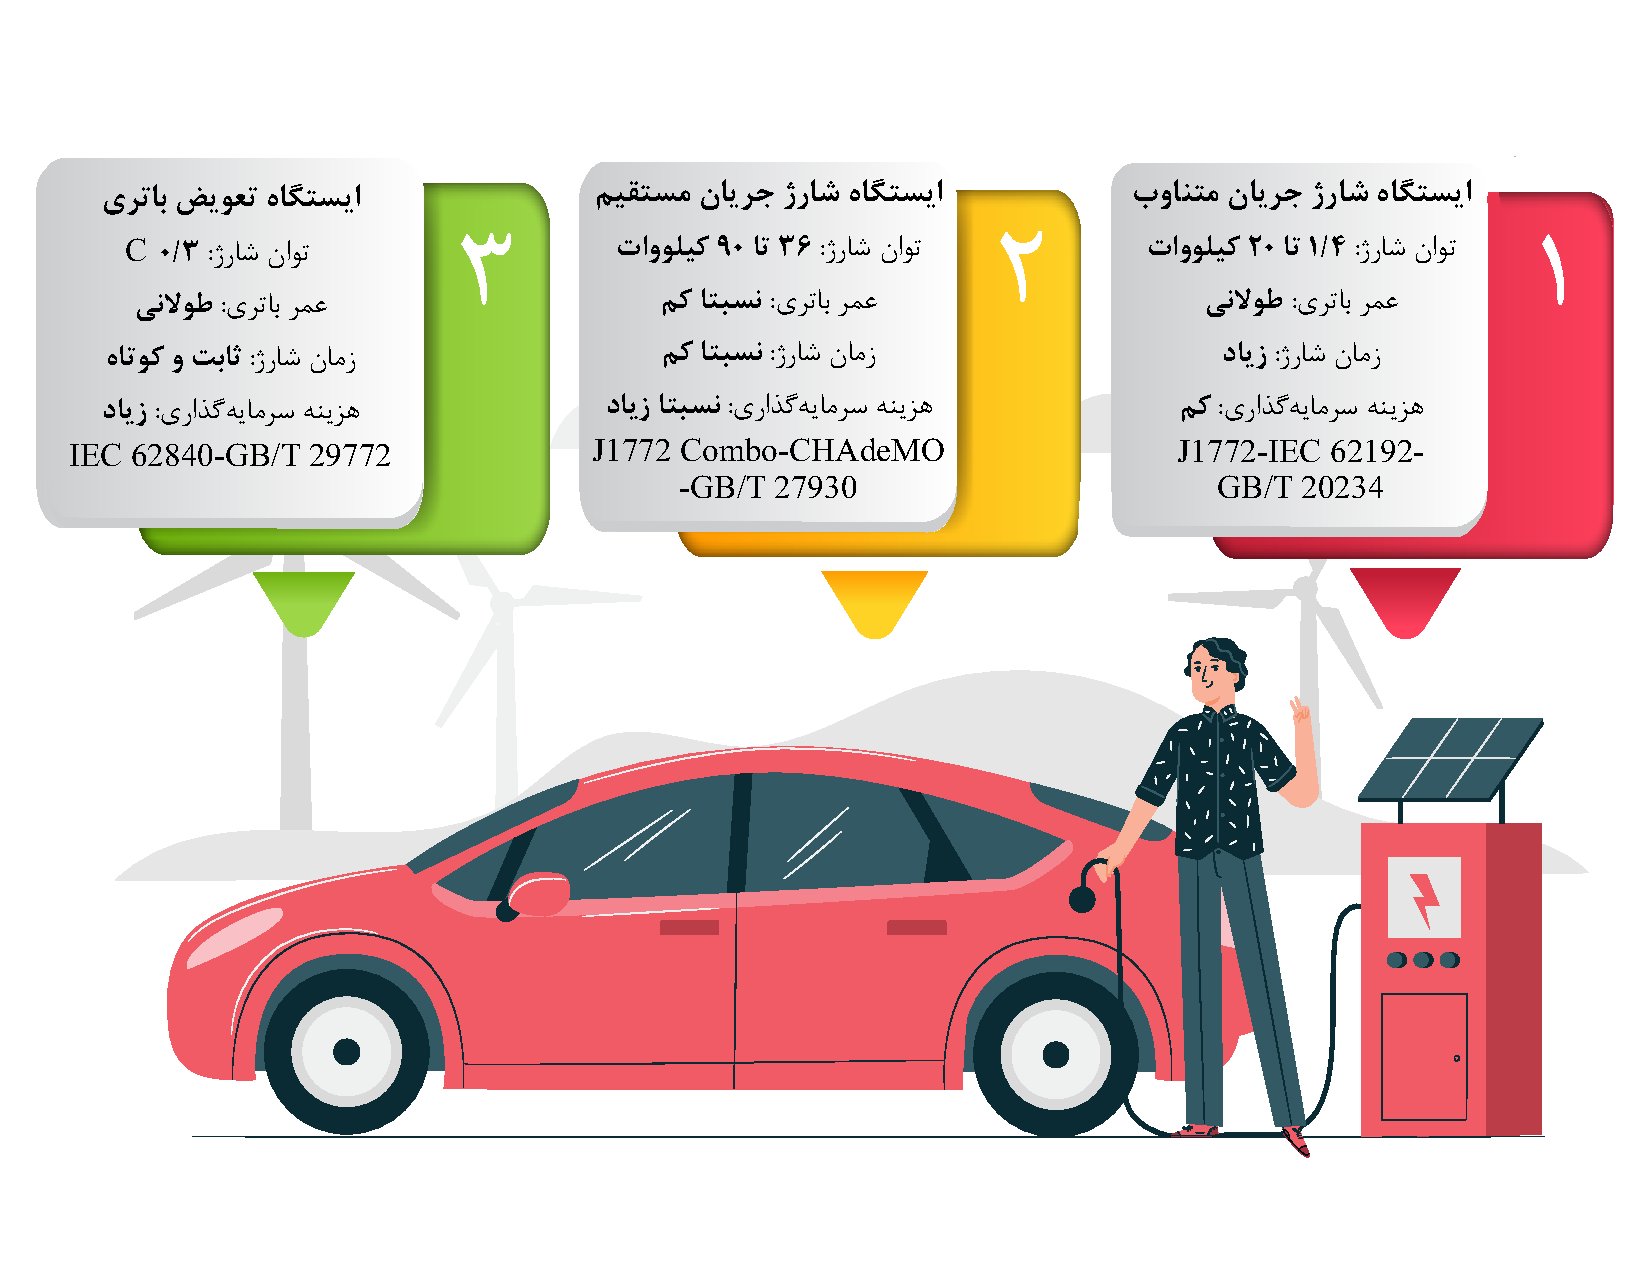
\includegraphics[width=0.8\textwidth]{U}
\caption{مقایسه ایستگاه‌های شارژی خودرو الکتریکی}
\label{figure}
\end{figure}


\section{تعاریف، اصول و مبانی نظری}
این قسمت ارائهٔ خلاصه‌ای از دانش کلاسیک موضوع است. این بخش الزامی نیست و بستگی به نظر استاد راهنما دارد.

\section{مروری بر ادبیات موضوع}
در این قسمت باید به کارهای مشابه دیگران در گذشته اشاره کرد و وزن بیشتر این قسمت بهتر است به مقالات ژورنالی سال‌های اخیر (۲ تا ۳ سال) تخصیص داده شود. به نتایج کارهای دیگران با ذکر دقیق مراجع باید اشاره شده و جایگاه و تفاوت تحقیق شما نیز با کارهای دیگران مشخص شود. استفاده از مقالات ژورنال‌های معتبر در دو یا سه سال اخیر، می‌تواند به اعتبار کار شما بیافزاید.

\section{نتیجه‌گیری}
‌در نتیجه‌گیری آخر این فصل، با توجه به بررسی انجام شده بر روی مراجع تحقیق، بخش‌های قابل گسترش و تحقیق در آن حیطه و چشم‌اندازهای تحقیق مورد بررسی قرار می‌گیرند.	در برخی از تحقیقات، نتیجه نهایی فصل روش تحقیق، ارائهٔ یک چارچوب کار تحقیقی 
\lr{(research framework)}
است.

	\begin{figure}[!htbp]
	\centering
	\begin{tikzpicture}[start chain=going right,>=latex,node distance=0pt]
	\node[draw,rectangle,on chain,minimum size=1.5cm] (rr) {};
	\node[draw,rectangle,on chain,draw=white,minimum size=1.3cm]{};
	% the rectangular shape with vertical lines
	\node[rectangle split, rectangle split parts=6,
	draw, rectangle split horizontal,text height=1cm,text depth=0.5cm,on chain,inner ysep=0pt] (wa) {};
	\fill[white] ([xshift=-\pgflinewidth,yshift=-\pgflinewidth]wa.north west) rectangle ([xshift=-15pt,yshift=\pgflinewidth]wa.south);
	\node at (wa.east) (A){};
	\draw [-latex] (A) --+(30:1.5) coordinate (B1);
	\draw [-latex] (A) --+(-30:1.5) coordinate (B2);
	% the circle
	\node [draw,circle,on chain,minimum size=1cm] at (B1) (se1) {$k_1$};
	\node [draw,circle,on chain,minimum size=1cm] at (B2) (se2) {$k_2$};
	\draw [-latex] (se1.east) --+(-25:1.65) coordinate (C1);
	\draw [-latex] (se2.east) --+(25:1.65) coordinate (C2);
	\node (O) at ($(C1)!0.5!(C2)$) {};
	\node [draw,circle,on chain,minimum size=3pt] at (O) (C3){};
	\draw [-latex] (C3)--+(0:2)node[right] {$\mu$};
	% the arrows and labels
	%   \draw[->] (se.east) -- +(20pt,0) node[right] {$\mu$};
	\draw[<-] (wa.west) -- +(-20pt,0) node[left] {$\lambda$};
	\node[align=center,below] at (rr.south) {};
	\node[align=center,below] at (wa.south) {};
	\node[align=center,below] at (se2.south) {};
	
	\end{tikzpicture}
	\caption{اجزای یک سیستم صف}
	\label{fig:queue}
\end{figure}






